%&pdfLaTeX
% !TEX encoding = UTF-8 Unicode
\documentclass{article}
\usepackage{ifxetex}
\ifxetex
\usepackage{fontspec}
\setmainfont[Mapping=tex-text]{STIXGeneral}
\else
\usepackage[T1]{fontenc}
\usepackage[utf8]{inputenc}
\fi
\usepackage{textcomp}

\usepackage{graphicx}
\usepackage{amssymb}
\usepackage[T2A]{fontenc}
\usepackage[russian]{babel}
\usepackage{fancyhdr}
\renewcommand{\headrulewidth}{0pt}
\renewcommand{\footrulewidth}{0pt}
\usepackage{color}

\definecolor{color17}{rgb}{0.21,0.37,0.57}
\definecolor{color18}{rgb}{0.31,0.51,0.74}

\begin{document}

\vspace{24pt}
\section*{{\large{}{\color{color17} \textbf{Глава 1. Прямое приближение 
Борна-Оппенгеймера.\label{HToc453749980}}}}}

\vspace{10pt}
\subsection*{{\large{}{\color{color18} \textbf{1.1 Приближение Борна-Оппенгеймера. 
Границы применимости.}}}}

\vspace{10pt}
\baselineskip=18pt
{\large{}Движение электрона в непроникающем ридберговском 
состоянии описывается его дальнодействующим 
взаимодействием с остовом, а именно, взаимодействием 
с кулоновским потенциалом, комбинированным 
с потенциалом свободно вращающегося диполя. 
Для анализа этого взаимодействия мы будем использовать 
приближение Борна-Оппенгеймера, применимое, 
когда диполь покоится или медленно движется 
по сравнению с движением электрона. Показано, 
что в данном приближении можно разделить радиальные 
и угловые переменные и в явном виде записать 
решение уравнения Шредингера для ридберговского 
электрона.}

\vspace{10pt}
{\large{}Сразу поговорим о границах применимости 
такого приближения. В прямом приближении Борна-Оппенгеймера 
момент импульса ридберговского электрона сильно 
связан с осью симметрии остова. Это имеет место, 
когда прецессия орбиты ридберговского электрона 
имеет более высокую частоту, чем вращение молекулы 
в целом.[8]}

\vspace{10pt}
%%\begin{figure}[htbp]
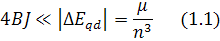
\includegraphics[width=165pt, height=31pt, keepaspectratio=true]{1-fig001.png}
%%\caption{This should be the caption for \texttt{1-fig001.png}.}
%%\end{figure}

\vspace{28pt}
{\large{}Здесь }

\includegraphics[width=10pt, height=19pt, keepaspectratio=true]{1-fig002.png}
{\large{} - вращательная константа в операторе центробежной 
энергии ядер}

\vspace{10pt}
%%\begin{figure}[htbp]
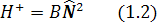
\includegraphics[width=118pt, height=20pt, keepaspectratio=true]{1-fig003.png}
%%\caption{This should be the caption for \texttt{1-fig003.png}.}
%%\end{figure}

\vspace{28pt}
{\large{}������ - полный момент молекулы (исключая 
спин ридберговского электрона), ������ - главное 
квантовое число, ������ - квантовый дефект.}

\vspace{10pt}
%%\begin{figure}[htbp]
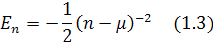
\includegraphics[width=160pt, height=34pt, keepaspectratio=true]{1-fig004.png}
%%\caption{This should be the caption for \texttt{1-fig004.png}.}
%%\end{figure}

\vspace{28pt}
%%\begin{figure}[htbp]
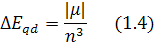
\includegraphics[width=116pt, height=35pt, keepaspectratio=true]{1-fig005.png}
%%\caption{This should be the caption for \texttt{1-fig005.png}.}
%%\end{figure}

\vspace{28pt}
{\large{}сдвиг энергии уровня.\label{HToc453749981}}

\vspace{10pt}
\subsection*{{\large{}{\color{color18} \textbf{1.2 Задача о ридберговском 
электроне в кулон-дипольном потенциале.}}}}

\vspace{10pt}
{\large{}С учетом дипольного взаимодействия мы 
можем записать гамильтониан ридберговской 
системы таким образом:}

\vspace{10pt}
%%\begin{figure}[htbp]
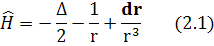
\includegraphics[width=161pt, height=35pt, keepaspectratio=true]{1-fig006.png}
%%\caption{This should be the caption for \texttt{1-fig006.png}.}
%%\end{figure}

\vspace{28pt}
{\large{}При выборе сферической системы координат, 
в которой ось z сонаправлена с направлением 
дипольного момента, уравнение Шредингера будет 
выглядеть так (используем атомную систему единиц):}

\vspace{10pt}
%%\begin{figure}[htbp]
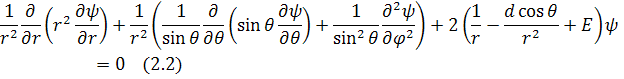
\includegraphics[width=468pt, height=59pt, keepaspectratio=true]{1-fig007.png}
%%\caption{This should be the caption for \texttt{1-fig007.png}.}
%%\end{figure}

\vspace{28pt}
{\large{}Разделим переменные }
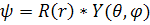
\includegraphics[width=113pt, height=19pt, keepaspectratio=true]{1-fig008.png}

\vspace{10pt}
%%\begin{figure}[htbp]
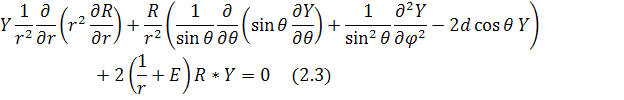
\includegraphics[width=468pt, height=75pt, keepaspectratio=true]{1-fig009.png}
%%\caption{This should be the caption for \texttt{1-fig009.png}.}
%%\end{figure}

\vspace{28pt}
{\large{}Введем функции }
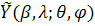
\includegraphics[width=71pt, height=20pt, keepaspectratio=true]{1-fig010.png}
{\large{}[8], которые удовлетворяют уравнению}

\vspace{10pt}
%%\begin{figure}[htbp]
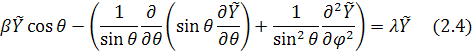
\includegraphics[width=354pt, height=41pt, keepaspectratio=true]{1-fig011.png}
%%\caption{This should be the caption for \texttt{1-fig011.png}.}
%%\end{figure}

\vspace{28pt}
%%\begin{figure}[htbp]
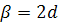
\includegraphics[width=44pt, height=19pt, keepaspectratio=true]{1-fig012.png}
%%\caption{This should be the caption for \texttt{1-fig012.png}.}
%%\end{figure}

\vspace{28pt}
{\large{}Теперь мы можем рассматривать отдельно 
уравнения на угловую и радиальную часть:}

\vspace{10pt}
%%\begin{figure}[htbp]
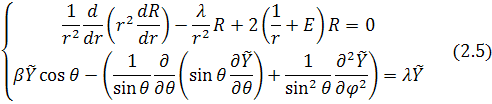
\includegraphics[width=369pt, height=78pt, keepaspectratio=true]{1-fig013.png}
%%\caption{This should be the caption for \texttt{1-fig013.png}.}
%%\end{figure}

\newpage

\end{document}
